\section{\todo{Dodecapolar RDTs}}

% Fill 9339
% https://logbook.cern.ch/elogbook-server#/logbook?logbookId=1081&dateFrom=2024-03-10T00%3A00%3A00&dateTo=2024-03-11T00%3A00%3A00
% http://localhost:8888/lab/workspaces/auto-Z/tree/work_afs2/jupyter/resonance_driving_terms/simulations/first_dodecapole_rdt/Plots.ipynb

During the commissioning of 2024, resonance driving terms measurements were performed by kicking the
beam at various strengths with the AC-Dipole at injection energy. Those measurements were intended
to measure several RDTs with a focus on decapoles.
However, a clear line in the vertical spectrum was observed at $5Q_y$, as shows
\cref{fig:high_orders:spectrum_dodecapole_5qy}. This line is contributed to by dodecapolar fields
(see \cref{appendic:rdts}) and is proportional to the vertical oscillation amplitude.

\begin{figure}[!htb]
    \centering
    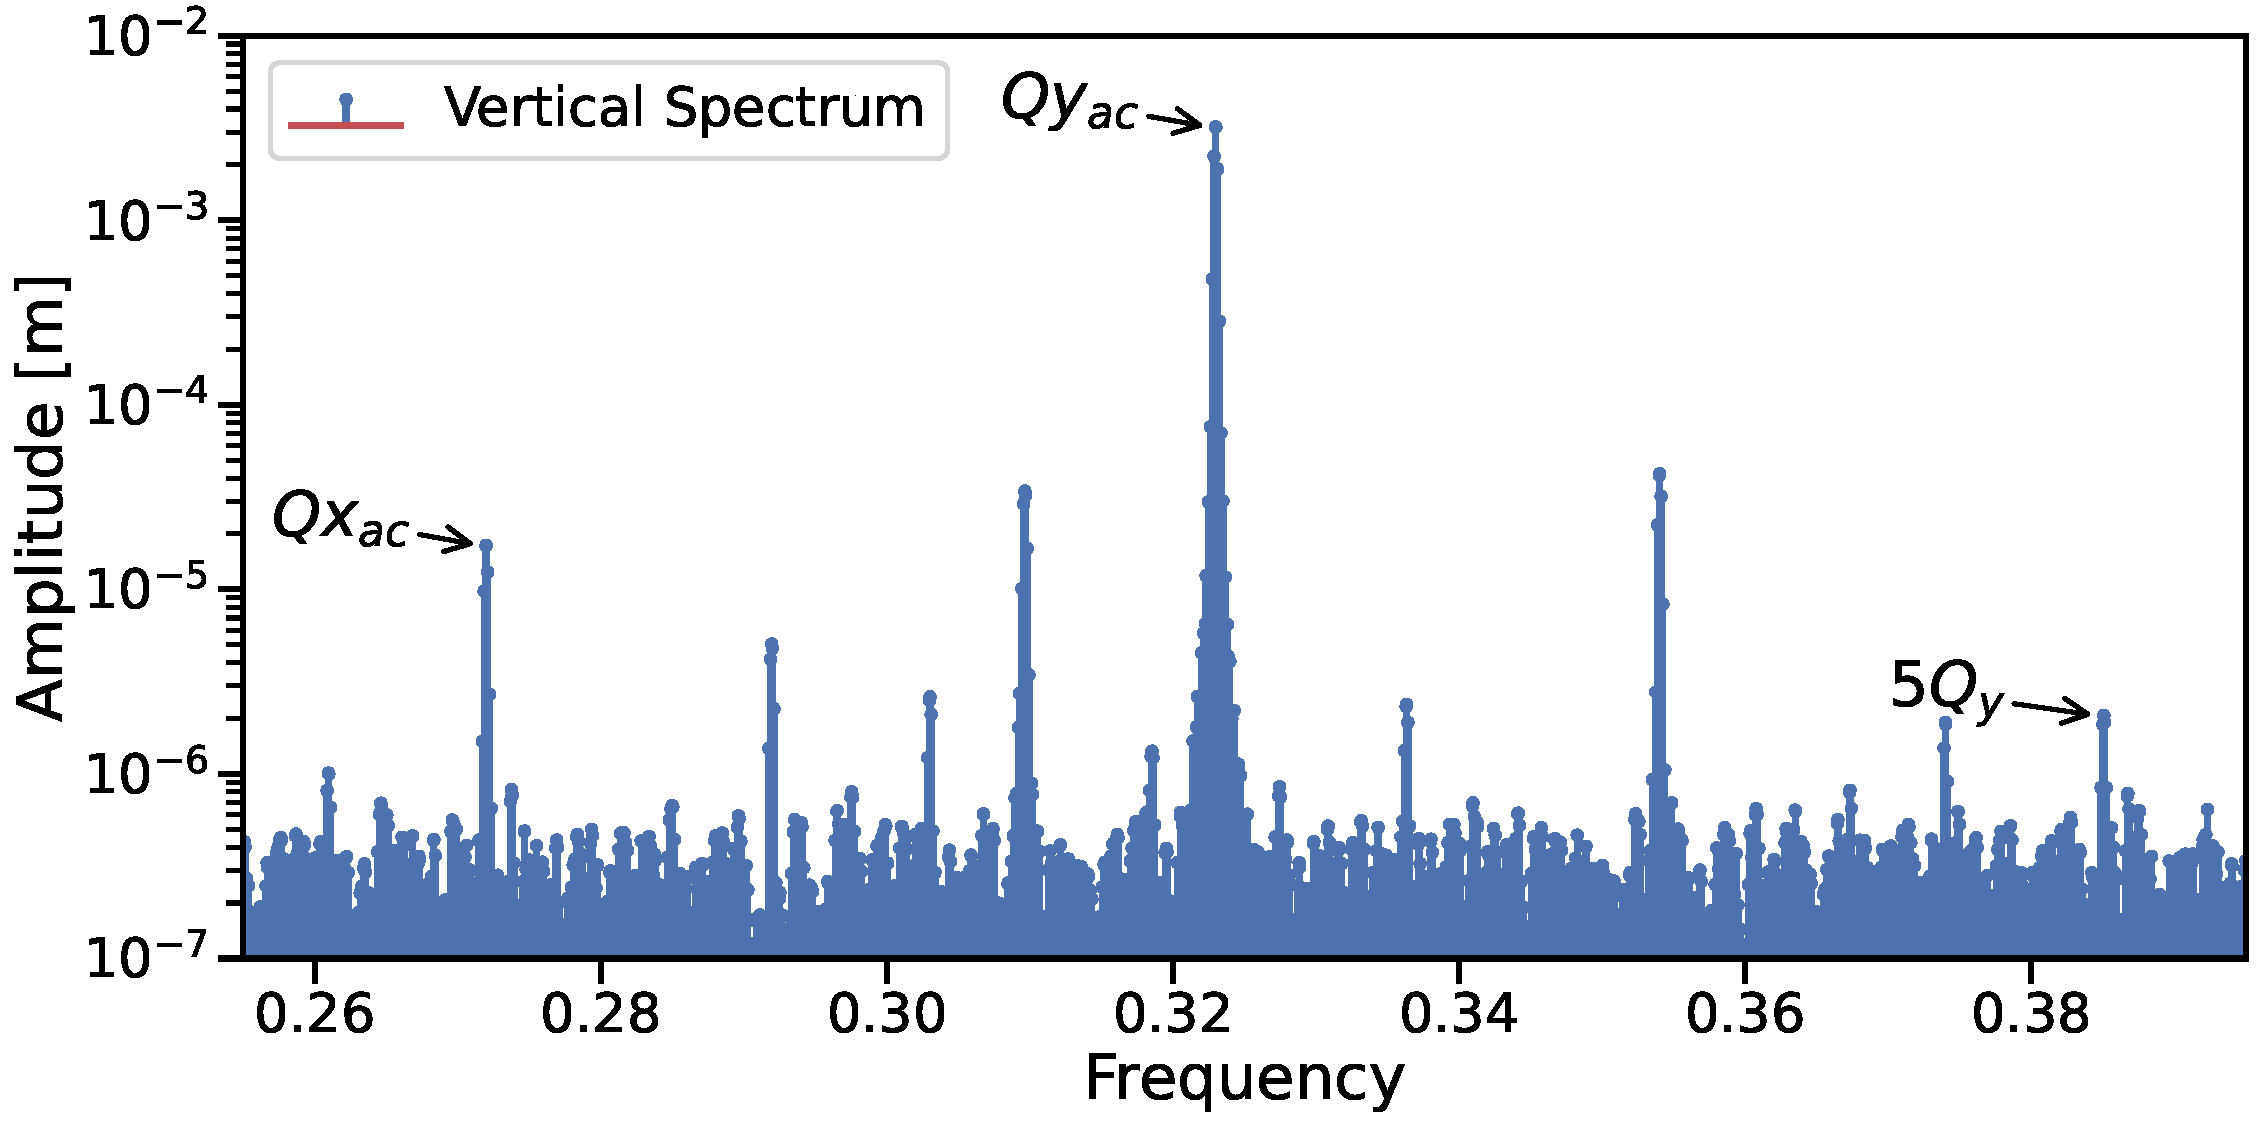
\includegraphics[width=0.8\textwidth]{./images/spectrum_dodecapole_5qy.pdf}
    \caption{Vertical spectrum of recorded turn-by-turn data for Beam 1 showing the tunes driven by the
    AC-Dipole along with a line contributed to by dodecapolar fields.}
    \label{fig:high_orders:spectrum_dodecapole_5qy}
\end{figure}

To achieve these measurements, the kick strength of the AC-Dipole was set up to $40\%$ of its
maximum, made possible by the newly introduced collimator sequence. The specific excited resonance
of the observed line is the $6Q_y$, related to the RDT $f_{0060}$.
\Cref{fig:high_orders:dodecapolar_f0060} highlights the real part of this RDT and the repeatability
of the measurement at varying kick strengths.

\begin{figure}[!htb]
    \centering
    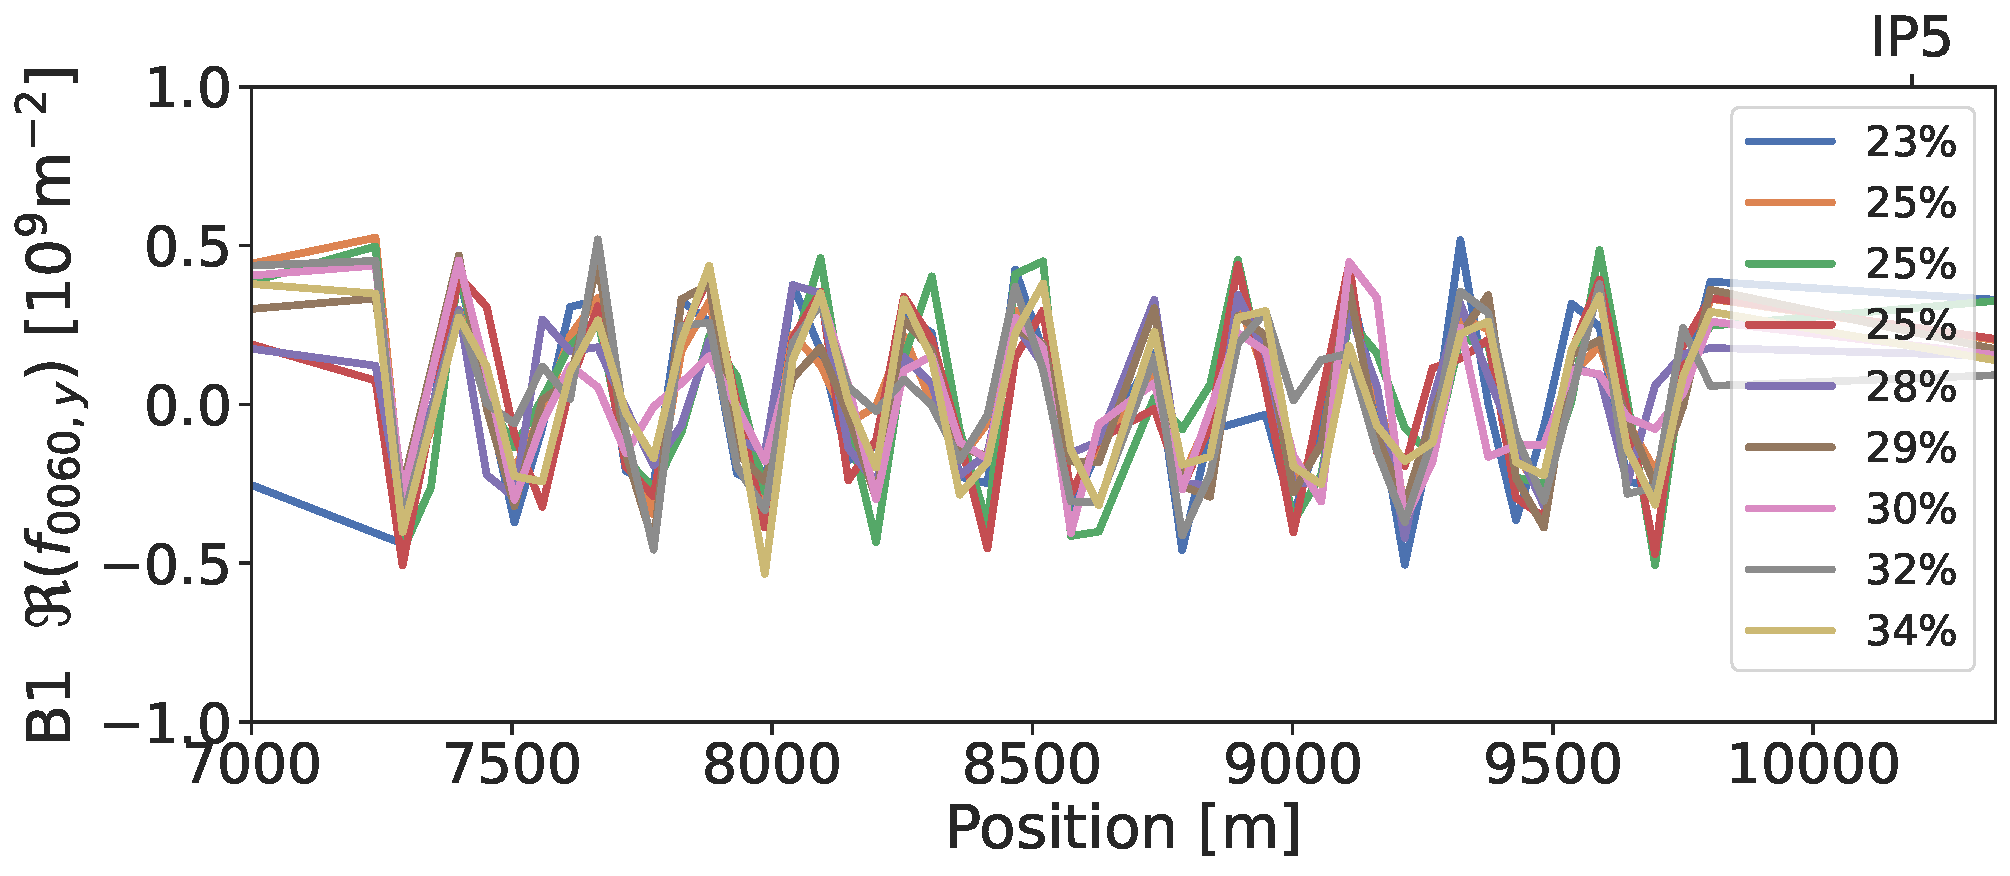
\includegraphics[width=0.8\textwidth]{./images/f0060y_all_meas_real.pdf}
    \caption{Real part of the dodecapolar RDT $f_{0060}$ measured with several kick strengths. The
    RMS amplitude is of $0.35\cdot10^{9}$.}
    \label{fig:high_orders:dodecapolar_f0060}
\end{figure}


